% ==========================================
% BAB I PENDAHULUAN
% ==========================================
\chapter{PENDAHULUAN}
\label{chap:pendahuluan}
% --- Latar Belakang ---
\section{Latar Belakang}
Perkembangan teknologi informasi yang semakin pesat dapat membawa manfaat besar bagi suatu organisasi maupun individu. Namun, di sisi lain juga dapat meningkatkan kerentanan terhadap serangan siber. Menurut \textit{World Economic Forum}, serangan siber dan kerentanannya berada di peringkat empat besar risiko utama yang dapat mengancam stabilitas global. Indonesia menjadi salah satu negara yang paling sering menjadi target serangan siber secara global. Berdasarkan laporan Badan Siber dan Sandi Negara (BSSN) pada Desember 2024, Indonesia menempati posisi lima besar negara paling sering diserang secara siber. Serangan utama yang terjadi meliputi \textit{ransomware}, \textit{phishing}, dan \textit{Distributed Denial of Service} (DDoS), yang menyasar infrastruktur penting nasional, institusi pemerintahan, dan sektor bisnis. Pada semester pertama tahun 2025, tercatat sebanyak 133{,}4 juta serangan siber di Indonesia, dengan serangan jenis \textit{Generic Protocol Command Decode} mendominasi sebanyak 68{,}37\%. Selain itu, serangan DDoS dan \textit{botnet} Mirai juga menjadi ancaman utama yang memengaruhi kestabilan dan keamanan sistem informasi di dalam negeri.

Salah satu ancaman siber yang semakin mengkhawatirkan adalah serangan yang berasal dari \textit{spyware}. \textit{Spyware} merupakan salah satu jenis \textit{malware} yang dirancang khusus untuk mengumpulkan data sensitif pengguna tanpa sepengetahuan mereka. Ada berbagai jenis \textit{spyware} yang umum ditemukan, antara lain \textit{keylogger} yang merekam aktivitas pengetikan keyboard, \textit{adware} yang menampilkan iklan secara agresif, serta \textit{trojan} yang memungkinkan akses jarak jauh ke perangkat korban. \textit{Spyware} modern semakin canggih dengan kemampuan menyembunyikan jejak dan beroperasi secara tersembunyi agar sulit dideteksi oleh sistem keamanan standar. Selain \textit{spyware} tipe \textit{file-based}, terdapat juga \textit{spyware fileless} yang bekerja langsung di memori (RAM) sehingga mampu menghindari teknik deteksi berbasis \textit{signature}. Salah satu contoh \textit{spyware} yang berbahaya adalah Pegasus, yang memiliki kemampuan infiltrasi tanpa interaksi pengguna (\textit{zero click exploit}) dan dapat mengakses berbagai jenis data pribadi serta mengendalikan perangkat secara \textit{remote} tanpa terdeteksi \autocite{reddy2024review}.

Dalam pengumpulan data intelijen siber, \textit{data crawling} merupakan proses otomatis yang memungkinkan pengambilan informasi dari berbagai sumber dalam skala besar dan sistematis. Proses ini melibatkan eksploitasi dan pengambilan data secara terus-menerus dari target, yang dapat berupa situs web, server, hingga perangkat yang terinfeksi \textit{malware}. Data yang dikumpulkan kemudian diproses secara lebih mendalam untuk memperoleh informasi relevan yang dapat digunakan dalam analisis ancaman \autocite{verma2021informationgathering}. Dalam konteks \textit{spyware} mode \textit{stealth}, \textit{data crawling} difasilitasi oleh \textit{spyware} yang mampu menyusup tanpa terdeteksi dan secara otomatis mengumpulkan data pengguna secara diam-diam.

Setelah data berhasil dikumpulkan, tahap eksfiltrasi menjadi proses kritis berikutnya, di mana data hasil pencurian dikirimkan secara tersembunyi ke server penyerang. Teknik eksfiltrasi yang digunakan dapat berupa trafik data terenkripsi, pemecahan data menjadi bagian kecil yang dikirim secara berkala untuk menghindari deteksi, atau penyamaran data dalam komunikasi normal jaringan.

Untuk menghadapi ancaman yang ditimbulkan oleh \textit{spyware}, upaya proteksi menjadi sangat penting dalam menjaga keamanan sistem dan data. \textit{Anti-spyware} adalah perangkat lunak yang dirancang untuk mendeteksi, mencegah, dan menghapus \textit{spyware}. Dalam menghadapi \textit{spyware} modern, terutama yang menggunakan teknik \textit{stealth} seperti \textit{fileless malware} yang berjalan langsung di memori, metode deteksi tradisional berbasis \textit{signature} dianggap kurang efektif.

Dalam penelitian ini, fokus utama terdapat pada tahap \textit{mission}, yaitu proses pengumpulan data (\textit{data crawling}) dan pengiriman data hasil pengintaian secara tersembunyi (\textit{eksfiltrasi}) oleh \textit{spyware} mode \textit{stealth}. Pelaksanaan \textit{data crawling} dan eksfiltrasi ini dilakukan untuk menguji kapabilitas \textit{anti-spyware} dalam mendeteksi aktivitas pengumpulan dan pengiriman data yang dilakukan secara diam-diam oleh \textit{spyware}. Dengan demikian, proses ini bertujuan untuk mengetahui efektivitas suatu sistem keamanan dalam menangkal aksi pencurian data intelijen siber yang tersembunyi dan sulit dideteksi.

% --- Rumusan Masalah ---
\section{Rumusan Masalah}
Berikut adalah rumusan masalah yang dibahas dalam tugas akhir: 
\begin{enumerate}
\item	Bagaimana cara mengimplementasikan mekanisme pengambilan data (\textit{crawling}) dan eksfiltrasi oleh \textit{spyware} mode \textit{stealth} dari sistem target tanpa terdeteksi oleh sistem keamanan?
\item	Bagaimana kinerja perangkat \textit{anti-spyware} dalam mendeteksi aktivitas \textit{data crawling} dan eksfiltrasi yang dilakukan oleh \textit{spyware} mode \textit{stealth}?
\end{enumerate}

% --- Tujuan ---
\section{Tujuan}
Berikut adalah tujuan dari pengerjaan tugas akhir: 
\begin{enumerate}
\item	Mengimplementasikan mekanisme pengambilan data dan eksfiltrasi oleh \textit{spyware} mode \textit{stealth} dari sistem target, serta menguji bagaimana proses tersebut dapat berjalan tanpa terdeteksi oleh sistem keamanan.
\item   Mengevaluasi kinerja perangkat \textit{anti-spyware} dalam mendeteksi aktivitas \textit{data crawling} dan eksfiltrasi yang dilakukan oleh \textit{spyware} mode \textit{stealth}, sehingga dapat diperoleh rekomendasi terkait efektivitas serta peningkatan sistem keamanan terhadap ancaman tersebut.
\end{enumerate}

% --- Batasan Masalah ---
\section{Batasan Masalah}
Batasan masalah dalam pelaksanaan tugas akhir adalah sebagai berikut: 
\begin{enumerate}
\item   Penelitian ini hanya berfokus pada pengujian kapabilitas deteksi \textit{anti-spyware} terhadap aktivitas \textit{data crawling} dan eksfiltrasi yang dilakukan oleh \textit{spyware} mode \textit{stealth} pada sistem operasi desktop.
\item   Evaluasi hanya mencakup perangkat \textit{anti-spyware} yang dipilih sesuai kriteria penelitian, tidak membandingkan seluruh produk \textit{anti-spyware} yang ada.
\item   Aktivitas \textit{data crawling} dan eksfiltrasi yang diujikan dilakukan dalam batasan jaringan dan topologi tertentu sesuai rancangan penelitian.
\item   Tugas akhir ini dikerjakan secara kelompok dengan anggota penelitian sebagai berikut:
  \begin{itemize}
      \item Nathaniel Liady
      \item M. Kasyfil Aziz
      \item Audra Zelvania Putri Harjanto
      \item Khayla Belva Annandira
  \end{itemize}
\end{enumerate}

% --- Metodologi Pengerjaan TA ---
\section{Metodologi}

\begin{figure}[H]
    \centering
    \captionsetup{justification=centering}
    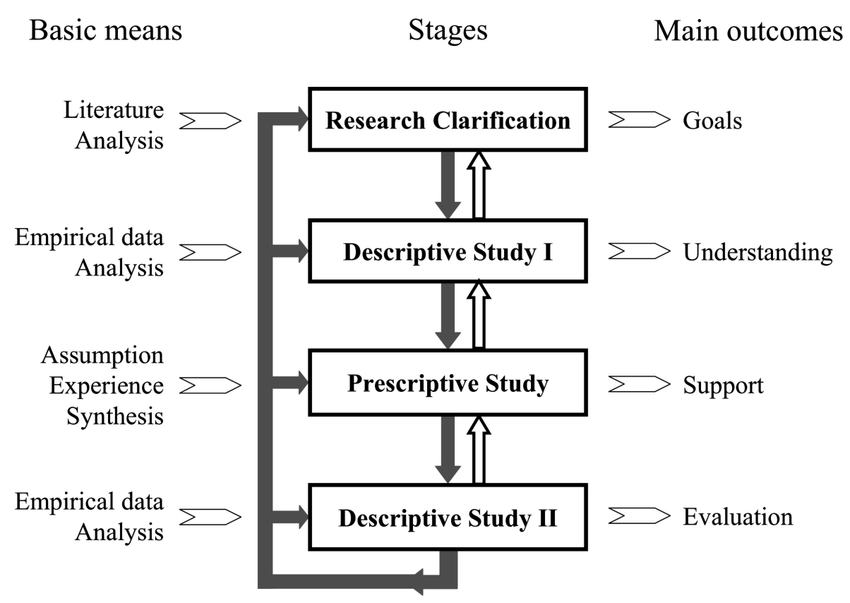
\includegraphics[width=0.85\textwidth]{image/drm-framework.png}
    \caption{Framework \textit{Design Research Methodology} (2009)}
    \label{fig:drm}
\end{figure}

Penelitian ini mengadopsi kerangka \textit{Design Research Methodology} (DRM)  yang dipublikasikan oleh Lucienne Blessing dan Amaresh Chakrabarti pada tahun 2009. Pendekatan ini memungkinkan penelitian dilakukan secara terstruktur mulai dari klarifikasi masalah hingga tahap evaluasi solusi. Dalam konteks tugas akhir ini, DRM digunakan untuk merancang dan mengevaluasi proses \textit{data crawling} dan \textit{data exfiltration} dalam \textit{spyware} mode \textit{stealth}. DRM terdiri dari empat tahapan utama, yaitu \textit{Research Clarification}, \textit{Descriptive Study I}, \textit{Prescriptive Study}, dan \textit{Descriptive Study II}.

\begin{enumerate}
    \item \textbf{\textit{Research Clarification (RC)}}  
    berfokus pada pemahaman awal mengenai permasalahan yang diteliti, ruang lingkup, serta tujuan penelitian. Pada tahap ini dirumuskan \textit{research questions} mengenai bagaimana mekanisme \textit{data crawling} dan eksfiltrasi dapat diimplementasikan dalam mode \textit{stealth} serta bagaimana perangkat \textit{anti-spyware} merespons aktivitas tersebut. Tahap RC menjadi dasar konseptual dalam merumuskan arah penelitian dan merancang kriteria keberhasilan evaluasi.

    \item \textbf{\textit{Descriptive Study I (DS-I)}}  
    bertujuan memperdalam pemahaman mendalam mengenai konteks, konsep, dan faktor-faktor yang berkaitan dengan permasalahan penelitian. Pada tahap ini dilakukan studi literatur untuk mengidentifikasi bagaimana proses yang diteliti dijelaskan dalam penelitian sebelumnya. Hasil analisis ini kemudian digunakan untuk menyusun \textit{reference model}, yaitu gambaran awal mengenai bagaimana proses yang diteliti dipahami menurut pengetahuan yang ada saat ini, yang nantinya menjadi dasar bagi perancangan solusi pada tahap berikutnya.

    \item \textbf{\textit{Prescriptive Study (PS)}}  
    berfokus pada perancangan solusi atau pendekatan yang akan dikembangkan untuk menjawab permasalahan penelitian. Berdasarkan pemahaman yang diperoleh dari tahap sebelumnya, pada tahap ini disusun rancangan konseptual yang menjelaskan bagaimana solusi tersebut diharapkan bekerja. Tahap ini menghasilkan \textit{impact model}, yaitu gambaran mengenai pengaruh yang diharapkan dari solusi yang dirancang terhadap proses atau sistem yang diteliti. Rancangan yang dihasilkan kemudian menjadi dasar bagi implementasi dan pengujian pada tahap berikutnya.

    \item \textbf{\textit{Descriptive Study II (DS-II)}}  
    digunakan untuk mengevaluasi solusi yang telah dirancang pada tahap sebelumnya. Pada tahap ini, solusi tersebut diimplementasikan dan diuji dalam kondisi yang direncanakan untuk melihat sejauh mana hasil aktual sesuai dengan harapan yang digambarkan dalam \textit{impact model}. Proses evaluasi ini bertujuan mengamati kinerja solusi, mengidentifikasi keberhasilan maupun keterbatasannya, serta menganalisis faktor-faktor yang memengaruhi hasil tersebut. Hasil dari DS-II digunakan untuk menilai efektivitas solusi secara menyeluruh dan memberikan dasar bagi penyempurnaan atau pengembangan studi lebih lanjut.
\end{enumerate}